\section{Maschinelles Lernen} \label{chpt:Stand_der_Technik_Maschinelles_Lernen}
Ein Teilgebiet der künstlichen Intelligenzen ist der Bereich des Maschinellen Lernens, welcher die Verarbeitung von Daten addressiert, um beispielsweise Vorhersagen in Situationen auf Basis von bestimmten Informationen zu treffen.
Im Jahr 1959 wurde dieser von Arthur Samuel geprägt, der die Herausforderung annahm, ein Schachspiel mit Hilfe einer Maschine zu lösen. (\cite[4]{joshi_machine_2020})
Das besondere hierbei ist das Erlernen des richtigen Lösungswegs, welcher nicht durch bestimmte Bedingungen gesteuert, sondern auf Basis verschiedener Informationen erlernt wird, die über diverse Quellen beigefügt werden.
Maschinelles Lernen findet in vielen Bereichen Anwendung, von Spracherkennung, Bilderkennung bis hin zu selbstfahrenden Kraftfahrzeugen. Diese Technologie wird zunehmend wichtiger in unserer immer vernetzteren Welt und trägt dazu bei, komplexer werdende Probleme zu lösen und immer innovativere Lösungen in verschiedenen Branchen einzuführen.

Im Wesentlichen geht es um die Entwicklung von Algorithmen, die dem Computer das Erkennen von Mustern und Zusammenhängen in Daten ermöglichen, wordurch ohne menschliche Intervention Aufgaben erledigt werden können.
Daher trainiert man Algorithmen auf Basis großer Datenbestände, um die erlernten Fähigkeiten auf neu erhobene Daten anzuwenden. Das Erlernen des nötigen Wissens basiert hierbei auf drei wesentlichen Faktoren, die die Qualität des Trainings beeinflussen. Neben den Informationen, die aus Daten gewonnen werden, nutzt man eine Kennzahl, die einen Vergleich zwischen dem aktuellen und idealen Verhalten herstellt, um mit dem dritten Faktor - einem Rückkopplungsmechanismus - das programm anzuleiten eine verbesserte Leistung in Folgeergebnissen zu erzielen. (\cite[4]{joshi_machine_2020})

Um ein Modell trainieren zu können, wird ein geeignetes künstliches Lernverfahren ausgewählt, das darauf abzielt, die Ausgaben eines künstlichen Systems in Bezug auf bestimmte Systemeingaben im Laufe des Lernprozesses zu optimieren. Unterschieden wird hautpsächlich in der Art und Weise, wie die 'Kritik' präsentiert wird, die zur Verbesserung des Verhaltens der jeweiligen künstlichen Systeme führen soll. Ein Training basiert auf sogenannten Hyperparametern, die Rahmenbedingungen des Prozesses festlegen. Dies kann zum Beispiel die Anzahl der Epochen, die Lern-Rate oder auch die Batch-Größe sein. Im Folgenden werden drei prägende Lernverfahren näher beschrieben.
\subsection{Überwachtes Lernen}\label{subsec:supervisedlearning}
Diese Art des Lernens (eng.: supervised learning) stellt einen wesentlichen Bereich des maschinellen Lernenes dar, um aus Informationen, bestehend aus Datenpunkten \textit{$X = x_1, x_2, \ldots, x_n$} mit einem zugehörigen Label aus \textit{$Y = y_1, y_2, \ldots, x_n$}, das nötige Wissen für bestimmte Anwendungsfälle zu erlangen. Anwendung findet dieses Verfahren in Systemen, die nicht-gelabelte Daten verarbeiten, um darauf basierend eine Vorhersage über die Zugehörigkeit abzugeben.
Mögliche Arten von neuronalen Netzwerken, die über diese Methode trainiert wurden, sind beispielsweise Bildklassifikatoren. Dabei ist es die Aufgabe des Modells $M$, basierend auf einen bestimmten Input $I$ mit Hilfe erlernter Muster und Zusammenhänge der Trainingsdaten eine Vorhersage über die Zugehörigkeit von $I$ zu treffen.
\begin{figure}[H]
	\hspace{-30mm}
	\centering
	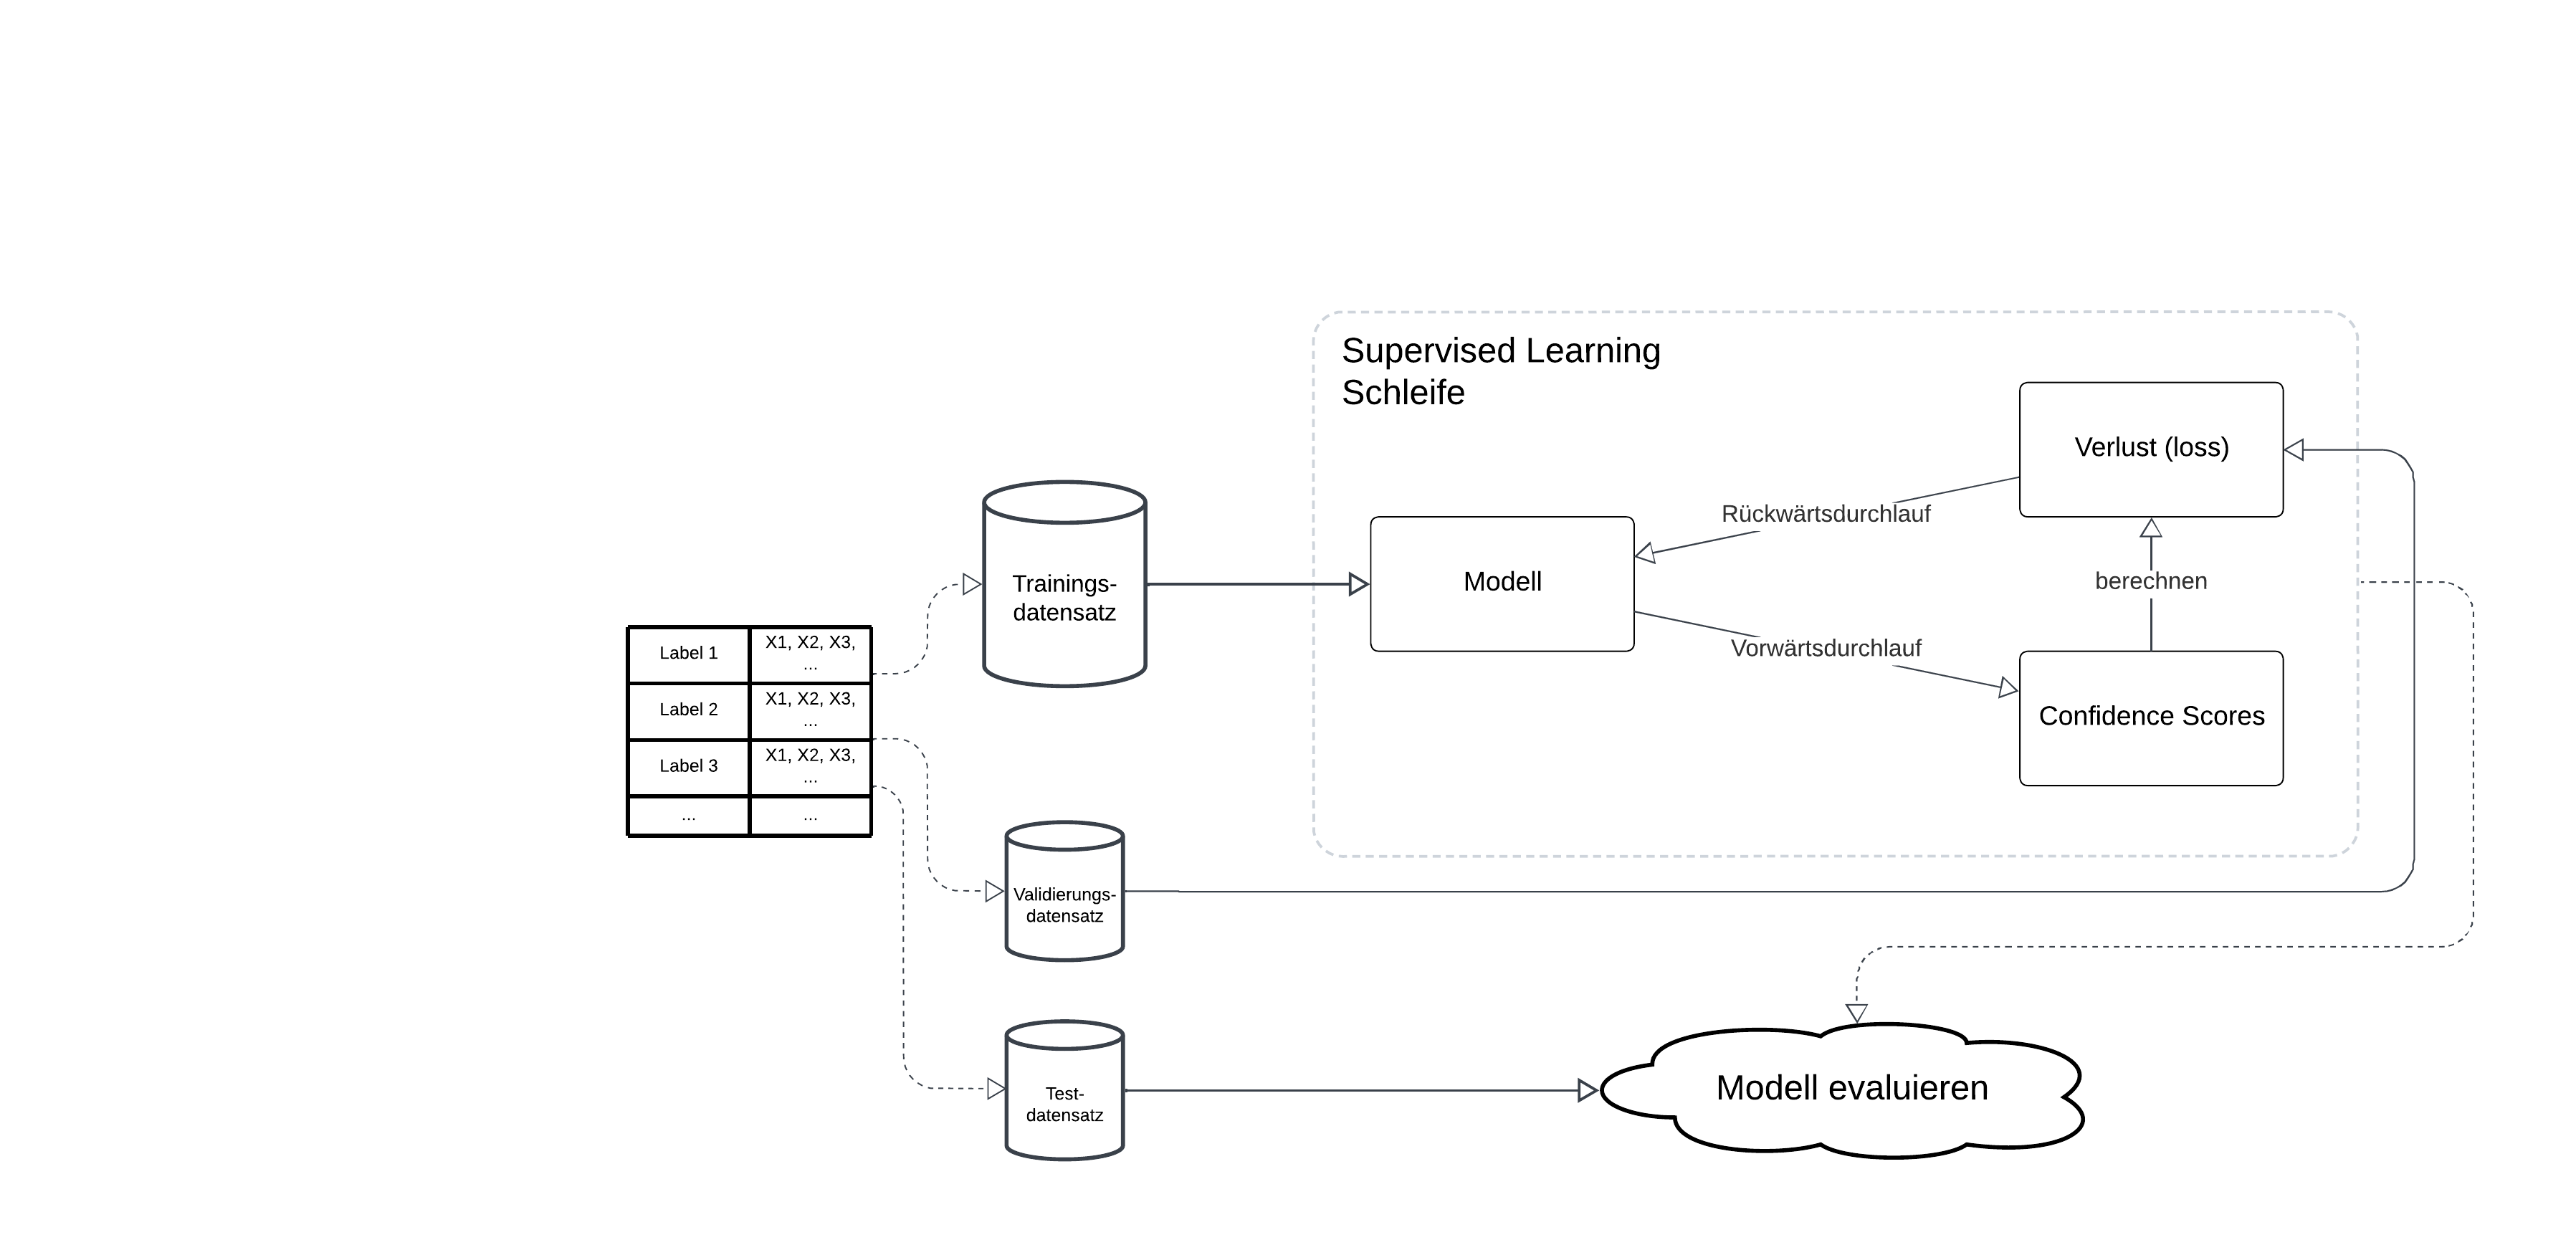
\includegraphics[width=0.8\linewidth]{Bilder/SupervisedLearning.png}
	\caption{Visualisierung grundlegender Prozesse während des Ablaufs eines überwachten Lernens}
\end{figure}
Der \textit{Ablauf} des Trainings lässt sich wie folgt beschreiben: nach Beenden von Datensammlung, Datenvorverarbeitung und Datensatztrennung in einen Trainings-, Validierungs- und Testdatensatz beginnt der eigentliche Teil des Trainings, wobei die Trainings- und Validierungsdaten für die aktualisierung der Modellparameter verwendet werden. Die Optimierung der Parameter wird auf Basis der Verlustfunktion mit Hilfe eines Rückwärtsdurchlaufes (eng.: Backward Propagation) durchgeführt, die mit der Differenz zwischen Vorhersagen des Modells aus dem Vorwärtsdurchlauf (eng.: Forward Propagation) und den realen Labeln berechnet wird.

Die \textit{Qualität} des Trainings wird meist anhand der Genauigkeit von Vorhersagen bestimmt, welche ausdrückt, wie gut die Klassifikation von im Training noch nicht gesehenen Daten funktioniert.
\[
\text{Accuracy} = \frac{\text{Anzahl korrekter Vorhersagen}}{\text{Gesamtanzahl der Vorhersagen}}
\]
 Weitere Metriken können die Präzision (eng.: Precision), der Recall oder auch der F1-Score sein. Neben Messungen der Modell-Genauigkeit kann man die Qualität des trainierten Modells auch anhand der Verlustfunktion (eng.: loss-function) oder der 'Area Under the Curve' (AUC), welche die Fläche unter der 'Receiver Operating Characteristic' (ROC) -- dem Verhältnis zwischen der True- und False-Positive-Rate -- messen.
\subsection{Unüberwachtes Lernen}
\begin{figure}[H]
	\centering
	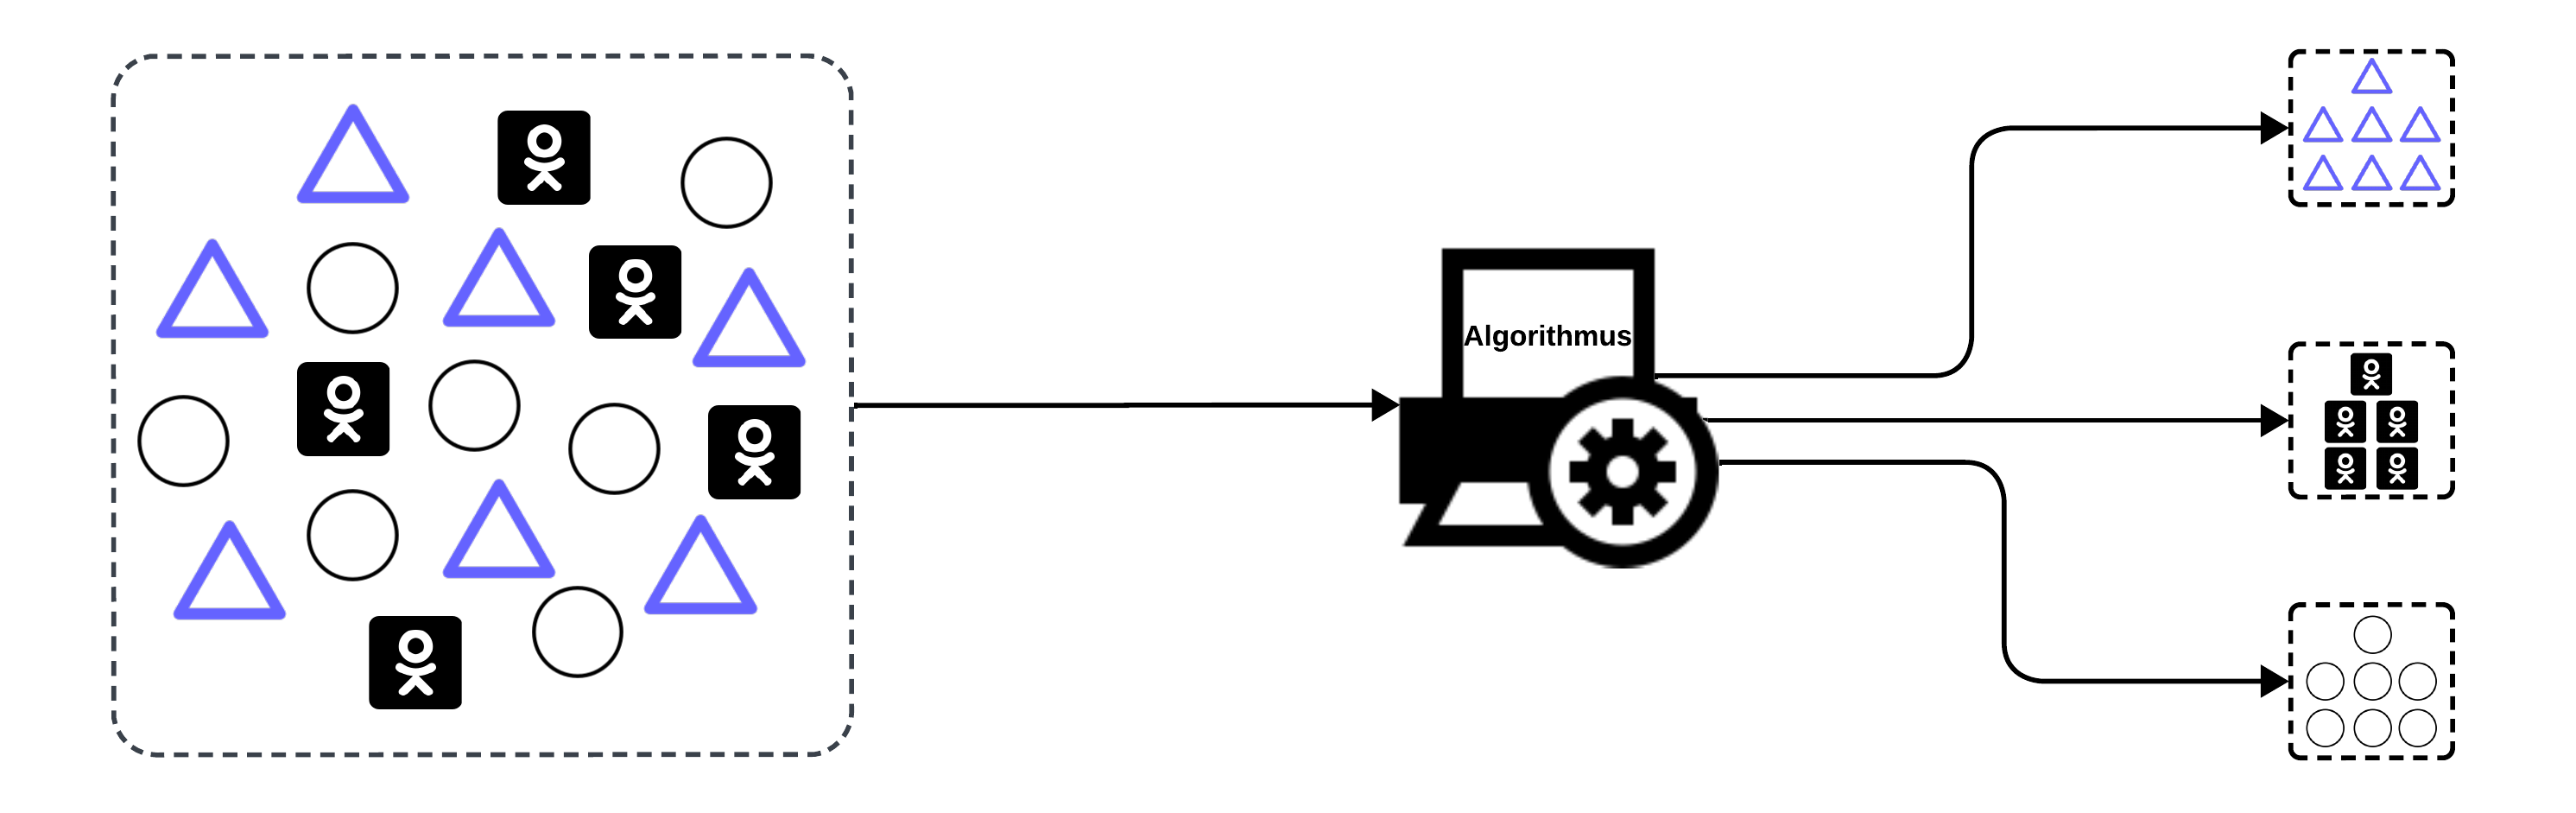
\includegraphics[width=0.8\linewidth]{Bilder/unsupervised_sample.png}
	\caption{Resultat eines auf unüberwachtem Lernen basierenden Clusterings}
\end{figure}
Unüberwachtes Lernen (eng.: unsupervised learning) stellt einen anderen bedeutenden Bereich im maschinellen Lernen dar, der sich von überwachtem Lernen (\ref{subsec:supervisedlearning}) dahingegen unterscheidet, dass keine expliziten Labels für die Trainingsdaten bereitgestellt werden. Diese Methode wird angewendet, wenn das Ziel darin besteht, Muster, Strukturen oder Zusammenhänge in den Daten zu entdecken, ohne dabei Kategorien oder Label vorzugeben, weshalb basierend auf Informationen eines Datensatzes, bestehend aus Datenpunkten \textit{$X = x_1, x_2, \ldots, x_n$} ohne dazugehöriges Label, trainiert wird. Das Modell soll dabei auf natürliche Art und Weise Strukturen, Muster und Zusammenhänge innerhalb der Eingabedaten ohne vorherige Kenntnisse der Zielvariable erlernen. \glqq Aufgabe ist es hier, passende Repräsentationen zu finden, die z. B. die Erkennung von Charakteristika in Datenmengen, Wiedererkennung von Ausnahmen oder die Erstellung von Prognosen ermöglichen.\grqq (\cite[5]{lorenz_reinforcement_2020}) Im Gegensatz zu Überwachtem Lernen (\ref{subsec:supervisedlearning}) geht es nicht um das Zurdnen von Mustern in vorhandenen Kategorien, sondern um das Auffinden von Clustern in einer bestimmten Datenmenge $X$. Dabei werden Modellparameter nicht über eine Verlustfunktion, die durch die Differenz zwischen tatsächlichem und vorhergesagtem Label berechnet wird, dargestellt, sondern die Parameter werden für die repräsentation inhärenter Muster in den Daten angepasst. Das Aufteilen des Datensatzes in 3 unabhängige Teile ist hierbei nicht notwendig, da keine Kategorien/Label für die jeweiligen Datenpunkte vorhanden sind. Es ist nur für die Auswertung des Algorithmus sinnvoll einen zweiten Datensatz zu erstellen, um damit die Qualität zu bewerten.
\begin{figure}[H]\label{img:unsupervisedworkflow}
	\hspace{-15mm}
	\centering
	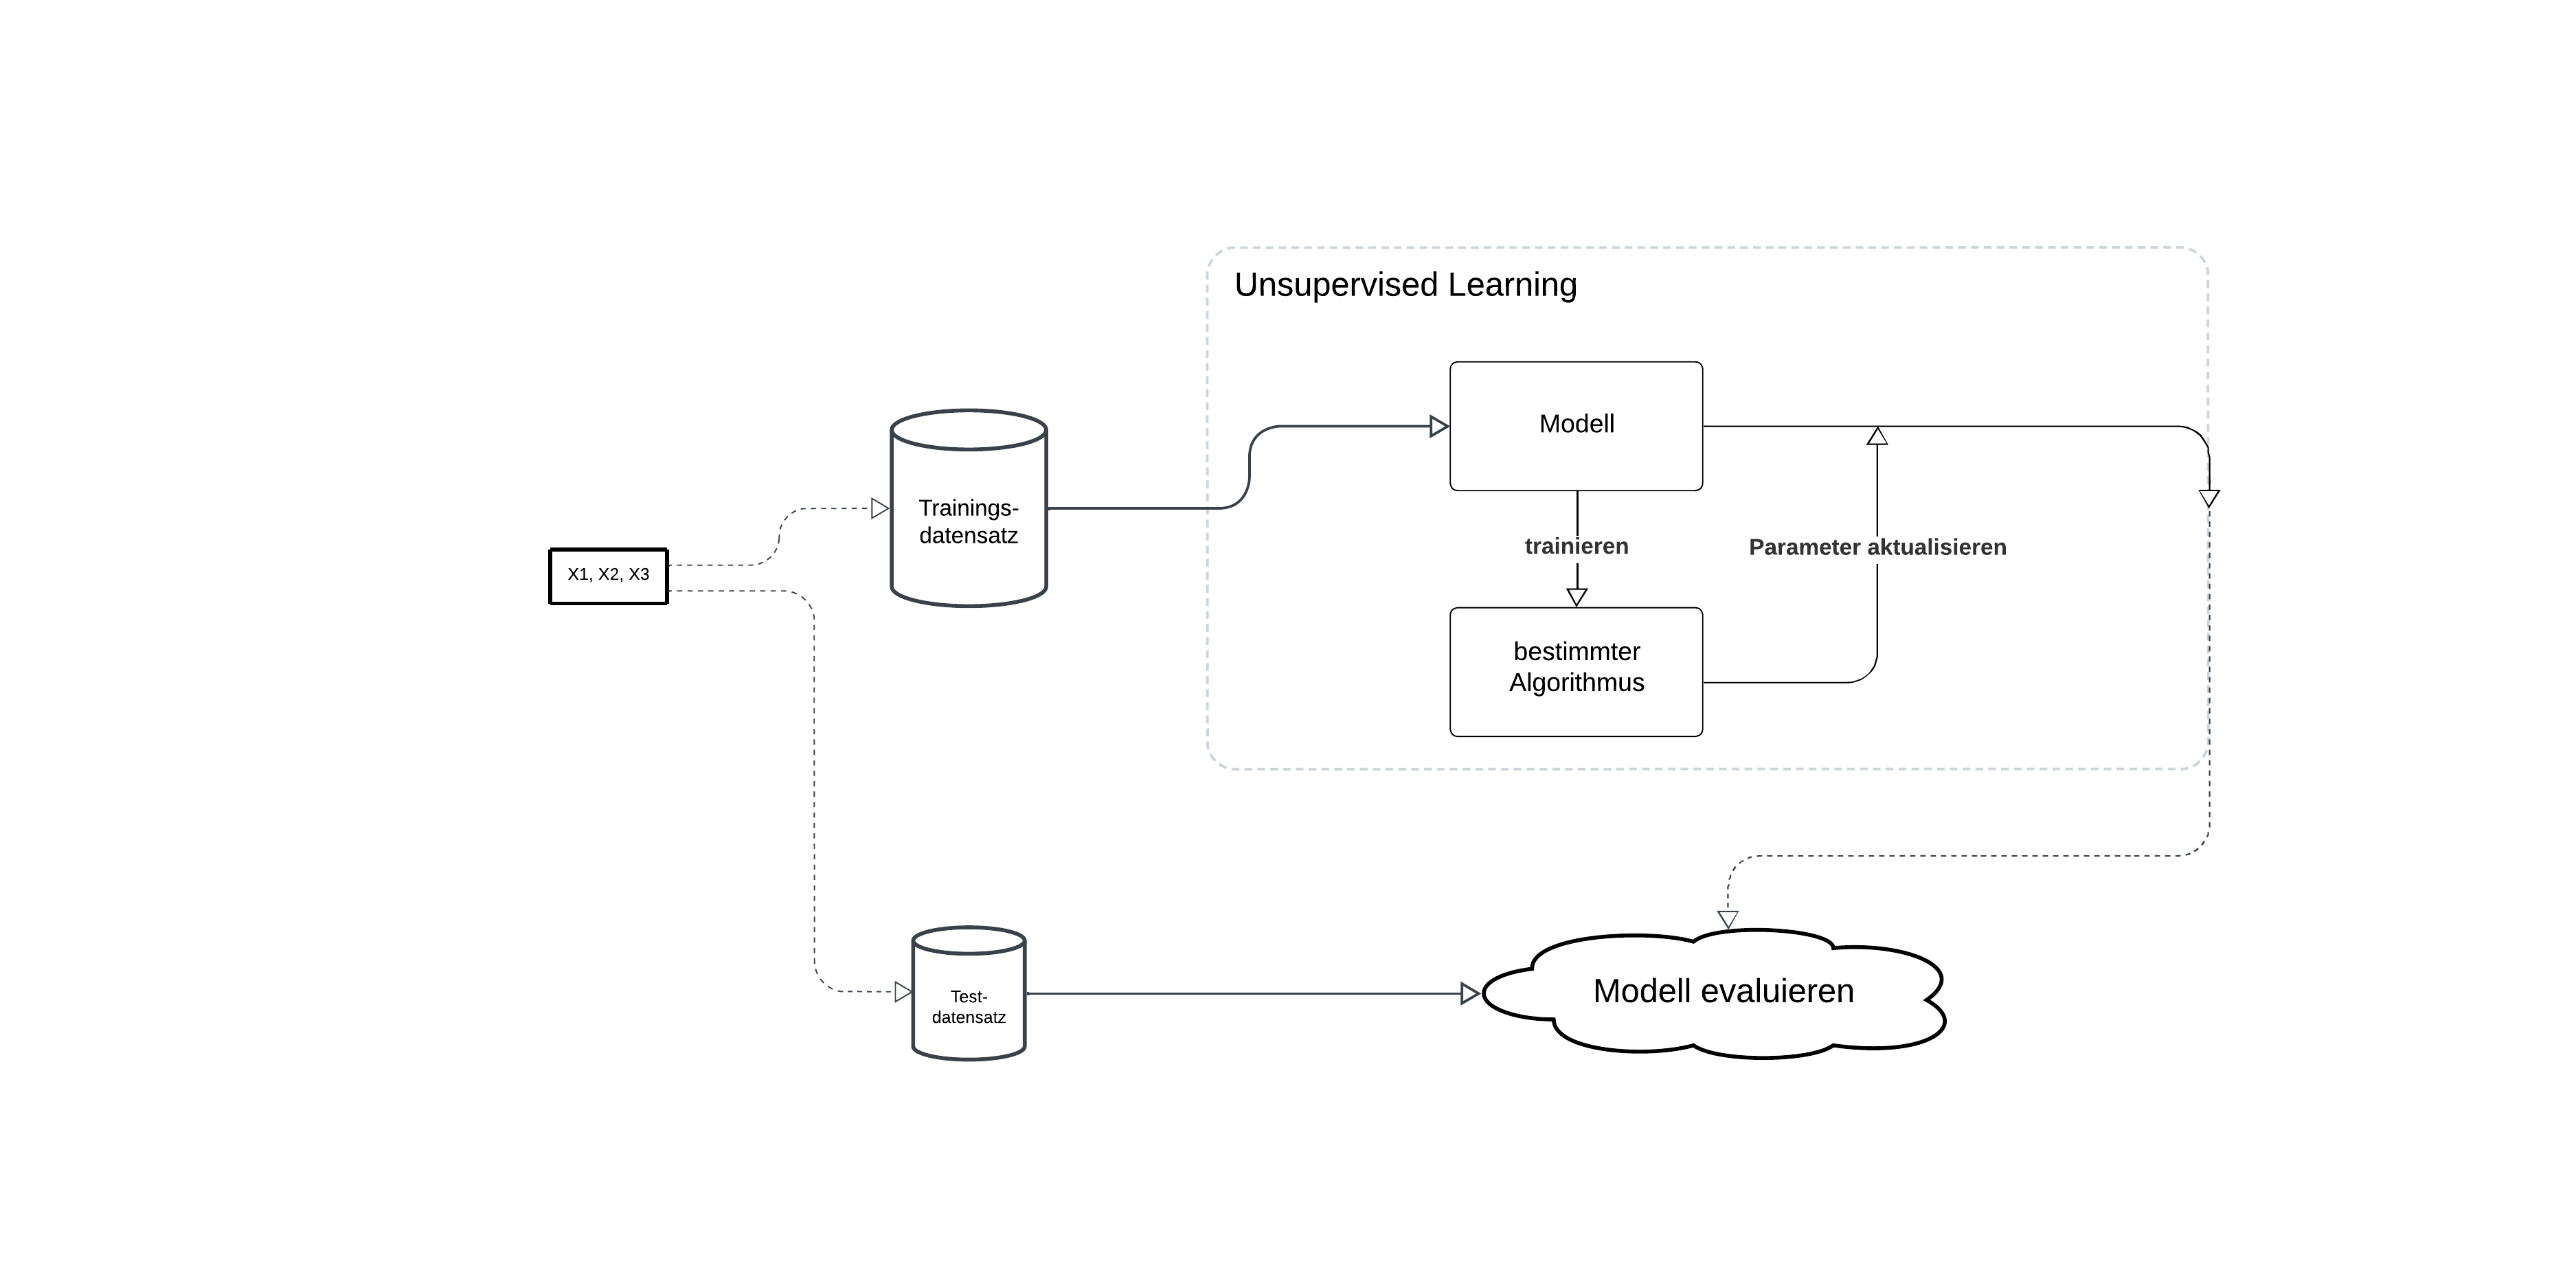
\includegraphics[width=0.8\linewidth]{Bilder/UnsupervisedLearning.png}
	\caption{Visualisierung grundlegender Prozesse während des Ablaufs eines unüberwachten Lernens}
\end{figure}
Der \textit{Ablauf} des Trainigs gestaltet sich wie folgt: Nach Abschluss von Datensammlung und Vorverarbeitung beginnt der eigentliche Prozess des unüberwachten Lernens. Im Gegensatz zum überwachten Lernen (\ref{subsec:supervisedlearning}) gibt es hierbei keine vordefinierten Zielvariablen. Den Datenpunkten $X = x_1, x_2, \ldots, x_n$ ist also initial keine Kategorie beziehungsweise kein Label zugeordnet, da die Menge $Y$ bist dato nicht existent ist. Im Gegensatz zu überwachtem Lernen nutzt man hier Algorithmen wie beispielsweise k-means Clustering, um eine bestimmte Operation auf den zu behandelnden Datensatz auszuführen. Mit Hilfe des Algorithmus wird ein bestimmtes Modell dahingehend trainiert, dass es einen bestimmten Datensatz zum Beispiel in bestimmte Kategorien unterteilen kann. Dafür analysiert der Algorithmus die jeweiligen Datenpunkte und versucht diese mit Hilfe von Zusammenhängen und verschiedenen extrahierten Merkmalen zu interpretieren. Anhand des dabei erlangten Wissens werden Modellparameter aktualisiert, wonach das unüberwachte Lernen beendet ist. Ein Ergebnis kann hierbei beispielsweise ein kategorisierter Datensatz sein.

Die  \textit{Qualität} eines Modells ist schwieriger zu messen als bei überwachtem Lernen \ref{subsec:supervisedlearning}, da keine klar definierte Zielvariable vorliegt, mit Hilfe welcher eine Genauigkeitsanalyse durchgeführt werden kann. Dennoch lässt sich auch dieses mit verschiedenen Metriken evaluieren. Zum einen kann man mit dem sogenannten Silhouette Score (\cite{shahapure_cluster_2020}) Clustering-Algorithmen evaluieren, da dieser das Zusammenpassen der verschiedenen Datenpunkte innerhalb eines Clusters bewertet. Je höher dieser Wert, desto besser sind die jeweiligen Cluster definiert. Neben Metriken, die durch bestimmte Berechnungen repräsentiert werden, lässt sich die Qualität eines Modells auch durch visuelle Methoden wie der Auswahl geeigneter Plots messen, die die Zugehörigkeit verschiedener Datenpunkte darstellen.
\subsection{Bestärkendes Lernen}